\chapter{Evaluación y resultados}\label{cap:resultados}\label{cap:experimentos}

Con los dieciséis algoritmos ya formulados en la Sección~\ref{cap:algoritmos}, este capítulo los somete al protocolo de evaluación
sin conexión y presenta los resultados publicados junto con una discusión honesta de lo que permiten y de lo que no
permiten concluir. El énfasis no está en declarar un ganador, sino en dejar trazable cada cifra
hasta el corpus, la semilla, el reparto y la configuración exactos que la produjeron.

La evaluación se ejecuta sobre la misma plataforma descrita en los capítulos anteriores: los
usuarios sintéticos, sus bibliotecas y el corpus gobernado viven en la misma base de datos que
sirve la aplicación.

\section{Fundamentos de evaluación}\label{sec:exp-fundamentos}

La parte más delicada no es implementar los algoritmos, sino evaluarlos de forma
comparable~\cite{herlocker2004evaluating, gunawardana2015evaluating}. La literatura señala
varios riesgos recurrentes: ajustar los hiperparámetros sobre el conjunto de prueba, comparar
algoritmos con repartos o candidatas distintos, medir solo la precisión y olvidar la
cobertura, la diversidad o la novedad, o extraer conclusiones sobre personas reales a partir
de simulaciones sintéticas. El trabajo de Cremonesi y otros mostró además que las métricas de
error sobre la valoración predicha y las métricas de acierto sobre la lista recomendada
pueden ordenar los algoritmos de forma distinta~\cite{cremonesi2010performance}. La respuesta
metodológica aceptada es fijar por adelantado, de forma inmutable, el corpus, el reparto, las
exclusiones, las métricas, las semillas y el presupuesto de ajuste, antes de comparar nada.
El protocolo de SavePoint deja la comparación preparada y repetible, pero no debe confundirse
con una afirmación sobre usuarios reales: los resultados de este capítulo se miden sobre un
corpus y una población sintética concretos.

Evaluar un recomendador sin usuarios reales exige fijar por adelantado cinco decisiones: la
tarea concreta que se mide (recomendar los siguientes \(K\) ítems que a una persona le
interesarán, no predecir la nota exacta que pondría), el criterio de relevancia que separa un
acierto de un fallo, el conjunto de candidatas sobre el que compite cada algoritmo, la división
de los datos entre lo que el modelo puede ver y lo que se usa para medir y la forma de agregar
el resultado por usuario en una única cifra por algoritmo. SavePoint fija estas decisiones en
un protocolo versionado antes de ejecutar la comparación.

La precisión en \(K\) mide qué proporción de los \(K\) ítems recomendados resultan relevantes;
la exhaustividad en \(K\) mide qué proporción de todos los ítems relevantes aparecen entre
esos \(K\). Ninguna de las dos distingue la posición dentro de la lista: acertar en el primer
puesto cuenta igual que acertar en el último. Para corregir esa carencia se usa la ganancia
acumulada descontada normalizada~\cite{jarvelin2002cumulated}, que descuenta el valor
de un acierto cuanto más abajo aparece y lo normaliza frente al orden ideal posible. La
precisión media promedia, para cada usuario, la precisión acumulada en cada posición
donde hubo un acierto y después promedia ese valor entre usuarios; es sensible tanto a la
cantidad de aciertos como a su posición.

Estas cuatro métricas comparten una limitación de fondo: ninguna equivale a satisfacción
humana, porque miden coincidencia con un historial pasado, no si a la persona le va a gustar lo
recomendado. Por eso se completan con tres métricas de otra naturaleza. La diversidad mide
cuánto se parecen entre sí los ítems de una misma lista recomendada; la novedad mide cuánto se
aleja la recomendación de lo obvio o ya muy popular; y la cobertura mide qué proporción del
catálogo llega a aparecer alguna vez recomendada. Un recomendador que maximiza solo precisión
o nDCG puede hacerlo a costa de las tres, recomendando siempre lo mismo a todo el mundo; la
Sección~\ref{cap:algoritmos} explica cómo SavePoint reordena sus listas para compensarlo.

\section{Protocolo de evaluación}\label{sec:exp-protocolo}

La evaluación publicada se ejecutó offline con el corpus congelado \texttt{2026.09.2} (190.479 obras
gobernadas, Sección~\ref{sec:datos-congelacion}) y el conjunto de
características \texttt{fs-v12-curated-tags-idf} (Sección~\ref{cap:algoritmos} y
Tabla~\ref{tab:pesos-familia}); la revisión posterior \texttt{fs-v13} no se ha evaluado. La población experimental contiene 400 usuarios de prueba sintéticos, generados de forma determinista; 79 cumplen la elegibilidad del split de prueba. La población se reparte en dos cohortes: \texttt{active\_history\_10\_to\_20}, con los 390 usuarios que tienen una biblioteca de entre 10 y 20 entradas y \texttt{no\_history}, con los 10 de arranque en frío, que no tienen ítems relevantes y no se evalúan; los 79 usuarios evaluables pertenecen todos a la primera. Los perfiles se generan a partir de nueve arquetipos: dos sin historial (diez usuarios), tres de perfil inicial (cien), tres de usuario normal (doscientos cuarenta) y uno intensivo veterano (cincuenta). Los arquetipos con historial tienen bibliotecas de entre 10 y 20 entradas y varían el número de géneros preferidos, la generosidad al puntuar y la mezcla de estados; llevan el marcador \texttt{synthetic-eval-user} para no contaminar el baseline de popularidad de la aplicación. El protocolo v15 fija semilla, versiones, snapshots, hashes, candidatas y exclusiones antes de consumir el test. La semilla permite reproducir esta ejecución, pero no sustituye un estudio de sensibilidad con múltiples semillas.

El protocolo publicado, v15, usa \emph{leave-fraction-out} por usuario, no
\emph{leave-one-out}: retiene varios ítems relevantes por persona en lugar de uno solo. Una
obra relevante es una entrada terminada o valorada con al menos siete medios puntos, con un
piso adicional de calidad externa (valoración agregada de origen de al menos 70 puntos) sobre
las candidatas a retener. Para cada usuario, el runner localiza su etiqueta de contenido con
más peso en el perfil y retira de ella un \(\lceil 0{,}3\times\) tamaño del grupo de esa
etiqueta\(\rceil\) de obras, nunca menos de una, retrocediendo de una en una si la retirada
desplazara esa etiqueta del primer puesto del perfil restante. Cuando ese mecanismo no se
puede construir para un usuario (sin ninguna señal de etiqueta de contenido, o sin candidatas
que superen el piso de calidad), el runner recurre al \emph{leave-one-out} simple de un único
ítem en lugar de excluir a esa persona del estudio; solo queda fuera quien no tiene ningún
positivo elegible en absoluto. Sobre los setenta y nueve usuarios evaluables, este mecanismo
retuvo doscientos dos ítems en total, una media de 2{,}56 por usuario con un rango de uno a
cinco. Todos los algoritmos reciben el mismo manifiesto de candidatas; el diseño evita
filtración de datos: ningún ítem retenido participa en la construcción del perfil, mientras que su
presencia entre las candidatas permite medir si se recupera.

Se calcula \(K\in\{5,10,20\}\). Si \(R_u\) es el conjunto relevante retenido de un usuario y
\(L_u^K\) los primeros \(K\) ítems de su lista, \(Precision@K=|L_u^K\cap R_u|/K\) y
\(Recall@K=|L_u^K\cap R_u|/|R_u|\). Al retener varios ítems por usuario, \(Recall@K\) deja de
ser binario y se convierte en una fracción continua, lo que aporta más información por
comparación que el \emph{leave-one-out} de una sola versión anterior del protocolo. El nDCG
y el MAP se calculan sobre la misma
lista. El protocolo también conserva diversidad
intra-lista, novedad, coberturas y concentración cuando el artefacto permite estimarlas.

\subsection{Reparto de los usuarios y uso de la validación}\label{sec:exp-reparto}

Los 400 usuarios sintéticos se reparten por usuario, no por ítem, en tres subconjuntos disjuntos con una semilla
fija: 240 de entrenamiento, 80 de validación y 80 de prueba (Tabla~\ref{tab:exp-reparto}). Las métricas de este
capítulo se calculan solo sobre los usuarios de prueba; dentro de cada uno de ellos, el protocolo v15 retira después
la fracción de ítems relevantes descrita arriba.

\begin{table}[htp]
\centering
\small
\begin{tabularx}{\textwidth}{ | L{0.17\textwidth} | C{0.17\textwidth} | Y | }
    \hline
    \textbf{Partición} & \textbf{Usuarios} & \textbf{Papel en este capítulo} \\
    \hline
    Entrenamiento & 240 & Población de referencia del filtrado colaborativo por vecinos (\texttt{cf-user-knn-v1}) y base de frecuencias con la que se mide la novedad. No se evalúan. \\
    \hline
    Validación & 80 & Reservada para seleccionar configuraciones; no se ha utilizado para ello (véase más abajo). \\
    \hline
    Prueba & 80 (79 evaluados) & Comparación final de las dieciséis variantes, con un único consumo por versión del protocolo. \\
    \hline
\end{tabularx}
\caption{Reparto de los 400 usuarios sintéticos y papel de cada partición.}
\label{tab:exp-reparto}
\end{table}

\textbf{Por qué solo 79 de los 400 usuarios se evalúan.} Los 79 no son una selección de los 400 por falta de datos:
son la partición de prueba, de 80 usuarios, menos uno que no tiene ningún ítem relevante elegible. El artefacto lo
registra como 80 solicitados, 79 evaluados y 1 omitido. Los otros 320 usuarios, 240 de entrenamiento y 80 de
validación, no se evalúan en la comparación final por diseño, no por ser inservibles.

\textbf{Ajuste de hiperparámetros.} El protocolo declaró, antes de ejecutar nada, una rejilla de ajuste de como
máximo 31 configuraciones que debía puntuarse solo sobre validación con \(nDCG@10\), para bloquear la ganadora antes
de tocar la prueba. No se conserva ninguna ejecución de esa rejilla: todos los artefactos conservados corresponden a
la partición de prueba y no hay ninguno sobre validación. Los parámetros de las dieciséis variantes (los pesos por
familia, el \(\lambda\) de la reordenación, los pesos de PopScore y los demás) son decisiones de diseño justificadas
en la Sección~\ref{cap:algoritmos}, no valores seleccionados sobre validación. Por tanto no se ajustó ningún
hiperparámetro mediante una búsqueda sobre la prueba, pero tampoco se utilizó la validación para ello.

Esto no equivale a un aislamiento completo de la prueba. El protocolo se modificó de v12 a v15 después de ver los
resultados de prueba de las versiones anteriores (Sección~\ref{sec:exp-evolucion}), de modo que el consumo único de la
partición de prueba rige dentro de cada versión del protocolo, no entre versiones. Es una limitación del estudio y se
recoge entre las amenazas a la validez (Sección~\ref{sec:exp-amenazas}).

\section{Evolución del protocolo: tres intentos, no uno}\label{sec:exp-evolucion}\label{sec:exp-v15-fidelidad}

Los números de versión de esta sección designan el \emph{protocolo} de evaluación, no el conjunto de
características (v15 se calculó con \texttt{fs-v12}, Sección~\ref{cap:algoritmos}). El protocolo se versiona con un
número entero que sube cada vez que un cambio impide comparar sus resultados con los
de las versiones anteriores. La Tabla~\ref{tab:exp-versiones} resume las versiones, reconstruidas a partir del
historial del repositorio y de los documentos de verificación. Hasta v14 el esquema de partición fue siempre
\emph{leave-one-out}, con un único ítem retenido por usuario; lo que cambió fue la señal de calidad, la regla de
elegibilidad de las candidatas, el elenco de algoritmos, la población sintética y el piso de calidad. Con los 400
usuarios se ejecutaron sobre la partición de prueba v12, v13, v14 y v15, pero la ejecución de v13 se descartó por un
error del banco de pruebas, no del protocolo (candidatas duplicadas en las listas ordenadas): los resultados válidos
son los de v12, v14 y v15.

\begin{table}[htp]
\centering
\small
\begin{tabularx}{\textwidth}{ | C{0.13\textwidth} | C{0.13\textwidth} | Y | }
    \hline
    \textbf{Versión} & \textbf{Fecha (2026)} & \textbf{Qué cambió} \\
    \hline
    v1--v2 & 7--8 sep. & Congelación inicial del contrato: \emph{leave-one-out} por usuario, \(K \in \{5, 10, 20\}\) y \(nDCG@10\) como métrica titular. La versión v2 limita las candidatas a obras con valoración. Primera ejecución de prueba, con la población inicial (26 de 40 usuarios de prueba evaluables). \\
    \hline
    v3--v6 & 9 sep. & Similitud de contenido por facetas y señal de calidad con confianza, calibradas en varias iteraciones; v6 es la versión que congeló el documento del protocolo. \\
    \hline
    v7--v9 & 9 sep. & Peso de PopScore de 0,20, valoración bayesiana (contracción hacia la media del corpus con \(m = 25\)) y regla de elegibilidad: obra gobernada, con fecha no futura, valoración de usuarios y al menos cinco valoraciones totales. \\
    \hline
    v10 & 10 sep. & Señal final de valoración (calidad por confianza), reordenación híbrida con MMR y rejilla de ajuste de 31 configuraciones. \\
    \hline
    v11--v12 & 10 sep. & Unificación de las etiquetas curadas y congelación de las entradas del cálculo. v12 es el primer cálculo completo con los 400 usuarios. \\
    \hline
    v13 & 11 sep. & Población sintética regenerada, con todas las bibliotecas con historial de entre 10 y 20 entradas. Su ejecución de prueba se descartó: un error del banco de pruebas duplicaba candidatas en las listas de los algoritmos de contenido y desbordaba sus métricas; se conserva marcada como inválida y no es un resultado. \\
    \hline
    v14 & 11 sep. & Piso de calidad externa para el ítem retenido. Segundo cálculo completo. \\
    \hline
    v15 & 12 sep. & \emph{Leave-fraction-out} sobre la etiqueta dominante de cada usuario. Versión publicada. \\
    \hline
\end{tabularx}
\caption{Versiones del protocolo de evaluación.}
\label{tab:exp-versiones}
\end{table}

Los resultados de v15 no fueron el primer cálculo ejecutado hasta el final contra la partición de prueba: lo precedieron v12 y v14, cada uno consumido una sola vez, con sus resultados conservados sin alterar. La forma concreta de v15 (retención por fracción sobre una etiqueta propia de cada usuario, piso de calidad externa, población con mínimo garantizado) responde a dos problemas reales que esos intentos dejaron medidos, no a una elección de diseño arbitraria.

\textbf{El protocolo v12 (10 de septiembre de 2026)} fue el primer cálculo congelado hasta el final. Su
resultado no fue una comparación entre algoritmos, sino un hallazgo metodológico: el
setenta y cuatro por ciento de los setenta y tres usuarios evaluables de aquella partición
(cincuenta y cuatro de setenta y tres) caía en un modo de \enquote{historial insuficiente} del
recomendador de contenido en cuanto el \emph{leave-one-out} uno retiraba su único positivo
elegible, porque la población sintética de entonces no garantizaba un mínimo de positivos
por biblioteca. En ese modo, las diez variantes de contenido y sus derivadas dejaban de usar
similitud de etiquetas y colapsaban a la misma ordenación por valoración y popularidad que ya
usaban los métodos de referencia, de modo que quince de los dieciséis algoritmos publicaron precisión,
recall, nDCG y MAP exactamente en cero. La prueba de Friedman fue significativa
(\(\chi^2=30{,}00\), \(p=0{,}0119\), \(n=73\)), pero ninguna de las ciento veinte
comparaciones por pares sobrevivió la corrección de Holm: bajo ese protocolo, ningún
algoritmo era declarable superior a otro. Se verificó que no era un fallo del código de
puntuación (los vectores de contenido coincidían byte a byte con la caché versionada y el
conjunto de candidatas era idéntico para los dieciséis algoritmos), sino una interacción entre
dos piezas congeladas por separado: el generador de población sintética y el umbral de
arranque en frío del recomendador de contenido.

Corregir esa interacción exigió dos cambios sucesivos. El primero (protocolo v13), con la población
rediseñada, amplió el tamaño de biblioteca sintética, ensanchó la franja de popularidad de
origen y garantizó un mínimo de cinco positivos elegibles por biblioteca. La ejecución de prueba de v13 no es
válida: un error del banco de pruebas duplicaba candidatas en las listas de los algoritmos de contenido (una obra
con varias etiquetas curadas aparecía varias veces) y desbordaba sus métricas, por lo que se descartó y se conservó
solo como evidencia del fallo. Por eso el efecto de la población rediseñada se midió en la ejecución de v14, que ya
reúne ambos cambios: el modo de historial insuficiente dejó de afectar a la partición de prueba y pasó del setenta y
cuatro por ciento de los usuarios a un cero por ciento. El segundo cambio añadió, sobre esa
población ya corregida, un piso de calidad externa (valoración agregada de origen de al menos
setenta puntos) al ítem que la retención de uno podía retirar, para que el positivo
retenido no dependiera solo del gusto personal simulado sino también de una señal de calidad
independiente, cerrando un sesgo de popularidad conocido en la literatura de evaluación de
recomendadores~\cite{cremonesi2010performance}.

\textbf{El protocolo v14 (11 de septiembre de 2026)}, con esos dos cambios ya aplicados, sí produjo un
ganador defendible: \texttt{hybrid-weighted-cf-v1} (\(nDCG@10=0{,}1526\)) y
\texttt{content-cbf-weighted-v1} (\(0{,}1452\)) superaron con significación a los métodos de referencia y
a \texttt{recency-v1}, con catorce de las ciento veinte comparaciones por pares significativas
tras Holm, frente a cero en v12 (\(\chi^2=105{,}28\), \(p=1{,}29\times10^{-15}\), \(n=79\)). La
diversidad intra-lista y la concentración de recomendaciones mejoraron en la misma medida: el
índice de concentración de Herfindahl-Hirschman (HHI) pasó de un rango de 0,55 a 0,71 en v12, propio
de un catálogo minúsculo de recomendaciones repetidas, a un rango de 0,005 a 0,03, consecuencia
directa de que el contenido ya no colapsaba a la misma alternativa de respaldo que los métodos de referencia. Aun
así, v14 seguía reteniendo un único ítem por usuario mediante retención de uno: cada
comparación por usuario solo podía acertar o fallar una vez, lo que limitaba cuántas
diferencias entre algoritmos podían alcanzar significación. El colaborativo puro, por ejemplo,
no llegó a diferenciarse de forma significativa de ningún otro algoritmo en v14, pese a tener
un nDCG@10 más bajo que las variantes de contenido con mejor combinación.

Ese límite de potencia estadística, no un defecto de v14, es lo que motivó el cambio final a
retención por fracción por etiqueta dominante propia de cada usuario que define el
protocolo v15: retener varios positivos por persona en lugar de uno solo da a cada comparación
más información por usuario sin necesidad de una población mayor. El resultado, ya presentado
en la Sección~\ref{sec:exp-significacion}, fue el esperado: de catorce comparaciones
significativas en v14 a cincuenta y cuatro en v15, con una diferenciación entre contenido y
colaborativo puro que v12 y v14 no tenían potencia estadística suficiente para establecer.
Los tres protocolos válidos y sus artefactos quedan versionados sin modificar (la ejecución descartada de v13 se
conserva aparte, marcada como inválida): v15 no invalida ni
reescribe los resultados de v12 o v14, los sustituye como publicación vigente por haber
corregido, de forma medida y documentada, los problemas que los dos intentos anteriores dejaron
al descubierto.

Conviene defender que v15 se acerca más a una prueba realista de lo que los algoritmos hacen, no que se ajusta para producir números más altos, porque corrige tres formas en las que v12 y v14 se apartaban de la literatura y del propio sistema. La primera es de encuadre: retirar y recuperar un subconjunto de valoraciones, en lugar de un único ítem, es la generalización natural del esquema \emph{All-but-N}, nombrado así desde Breese, Heckerman y Kadie~\cite{breese1998empirical} y sistematizado por Herlocker et al.~\cite{herlocker2004evaluating}, del que el \emph{leave-one-out} de los protocolos v6 a v14 (Tabla~\ref{tab:exp-versiones}) es el caso \(N=1\); v15 solo calcula \(N\) por usuario, en proporción al tamaño de su grupo de obras con la etiqueta dominante. La segunda es de fidelidad a la señal que el sistema usa: \texttt{facet\_similarity()}, el código de puntuación de los dieciséis algoritmos, combina cada familia de faceta como una suma ponderada, nunca como un único rasgo ganador, de modo que el 21{,}3\,\% de los casos verificados antes de congelar el protocolo en los que la etiqueta retirada deja de ser la primera del perfil recalculado no invalida la prueba: el perfil sigue apoyándose en ella con menos peso~\cite{pazzani2007content} y exigir lo contrario habría excluido usuarios que el sistema sí atiende. La tercera es de inclusión: el usuario para el que el mecanismo por fracción no se puede construir cae al \emph{leave-one-out} simple en lugar de quedar fuera, lo que evita quedarse solo con los usuarios más fáciles de evaluar y llamar a eso representativo.

Ninguno de los tres argumentos convierte v15 en evidencia sobre jugadores reales, como recuerda la Sección~\ref{sec:exp-amenazas}. Lo que establecen es que, dentro de la simulación, v15 mide la pregunta que se propone medir (¿recupera el sistema contenido afín al gusto que la propia biblioteca del usuario ya demuestra?) con más fidelidad al mecanismo de puntuación real y con menos artefactos de diseño heredados que v12 o v14, no solo con mejores cifras.

\section{Resultados publicados}\label{sec:exp-resultados}\label{sec:exp-exito}

La Tabla~\ref{tab:resultados-ndcg10} resume \(nDCG@10\), MAP@10 y el tiempo de pared de cada algoritmo, en segundos, tal como los registra el artefacto v15. Las métricas son las de los 79 usuarios evaluables, que pertenecen a la cohorte \texttt{active\_history\_10\_to\_20}; esa cohorte no es el conjunto de los 79, sino los 390 usuarios sintéticos con una biblioteca de entre 10 y 20 entradas; solo se evalúan los 79 que caen en la partición de prueba y tienen al menos un ítem relevante elegible. El tiempo es la duración del proceso que ejecutó cada algoritmo, no un tiempo por usuario. Se muestra una tabla compacta para evitar repetir cuatro métricas por tres valores de \(K\); el artefacto versionado \texttt{evaluation-400-test-2026-09-12-v15.artifact.json} y su transcripción en \texttt{docs/verification/evaluation-cohorts-400-test-2026-09-12-v15.md} preservan la transcripción completa para \(K=5,10,20\).

\begin{table}[H]
\centering
\caption[Resultados v15 publicados para los 79 usuarios evaluables]{Resultados v15 publicados (conjunto de características \texttt{fs-v12}) para los 79 usuarios evaluables de la cohorte \texttt{active\_history\_10\_to\_20}, con el tiempo de pared de cada algoritmo en segundos. No son resultados con usuarios reales.}\label{tab:resultados-ndcg10}
\small
\renewcommand{\arraystretch}{1.2}
\setlength{\tabcolsep}{3pt}
\begin{tabularx}{\textwidth}{@{}>{\ttfamily\footnotesize\raggedright\arraybackslash}p{0.385\textwidth}Y>{\raggedleft\arraybackslash}p{0.105\textwidth}>{\raggedleft\arraybackslash}p{0.105\textwidth}>{\raggedleft\arraybackslash}p{0.105\textwidth}@{}}
\textnormal{Algoritmo} & \textnormal{Familia} & \textnormal{\footnotesize nDCG@10} & \textnormal{\footnotesize MAP@10} & \textnormal{\footnotesize Tiempo (s)} \\
\hline
random-v1 & referencia & 0,00000 & 0,00000 & 25,1 \\
popularity-v1 & referencia & 0,00340 & 0,00098 & 5,1 \\
content-cbf-weighted-v1 & contenido & 0,17245 & 0,10878 & 492,8 \\
content-cbf-multiplicative-v1 & contenido & 0,08558 & 0,05934 & 491,4 \\
content-cbf-twostage-v1 & contenido & 0,11724 & 0,06767 & 488,5 \\
content-cbf-neg-v1 & contenido & 0,11778 & 0,07368 & 488,2 \\
content-cbf-weighted-pop-v1 & contenido + popularidad & 0,15181 & 0,09826 & 484,0 \\
content-cbf-multiplicative-pop-v1 & contenido + popularidad & 0,08517 & 0,05898 & 480,4 \\
content-cbf-twostage-pop-v1 & contenido + popularidad & 0,11410 & 0,06551 & 484,2 \\
content-cbf-neg-pop-v1 & contenido + popularidad & 0,09936 & 0,06134 & 483,9 \\
recency-v1 & contenido + novedad & 0,00594 & 0,00422 & 427,6 \\
content-cbf-mmr-v1 & contenido + diversidad & 0,13888 & 0,08685 & 483,3 \\
content-cbf-mmr-pop-v1 & contenido + diversidad & 0,13824 & 0,09353 & 481,7 \\
cf-user-knn-v1 & colaborativo & 0,02098 & 0,01099 & 16,8 \\
hybrid-weighted-cf-v1 & híbrido & 0,16989 & 0,10758 & 439,7 \\
hybrid-mmr-v1 & híbrido + diversidad & 0,15913 & 0,09741 & 493,1 \\
\end{tabularx}
\end{table}

La Tabla~\ref{tab:ndcg-todos-k} conserva \(nDCG\) en los tres cortes solicitados para el catálogo completo de variantes v15. Precision, recall y MAP permanecen en el artefacto y en la matriz de algoritmos para evitar una tabla de dieciséis filas y doce métricas que perdería legibilidad.

\begin{table}[H]
\centering
\caption{nDCG publicado por algoritmo y corte $K$ en v15 (\texttt{fs-v12}).}\label{tab:ndcg-todos-k}
\tablecompact
\begin{tabularx}{\textwidth}{@{}>{\ttfamily\raggedright\arraybackslash}p{0.45\textwidth}Yrrr@{}}
\textnormal{Algoritmo} & \textnormal{Familia} & \textnormal{$K=5$} & \textnormal{$K=10$} & \textnormal{$K=20$} \\
\hline
random-v1 & referencia & 0,00000 & 0,00000 & 0,00000 \\
popularity-v1 & referencia & 0,00191 & 0,00340 & 0,00340 \\
content-cbf-weighted-v1 & contenido & 0,14114 & 0,17245 & 0,18987 \\
content-cbf-multiplicative-v1 & contenido & 0,07707 & 0,08558 & 0,10241 \\
content-cbf-twostage-v1 & contenido & 0,08827 & 0,11724 & 0,14002 \\
content-cbf-neg-v1 & contenido & 0,09656 & 0,11778 & 0,12992 \\
content-cbf-weighted-pop-v1 & contenido + popularidad & 0,13179 & 0,15181 & 0,17409 \\
content-cbf-multiplicative-pop-v1 & contenido + popularidad & 0,07677 & 0,08517 & 0,10200 \\
content-cbf-twostage-pop-v1 & contenido + popularidad & 0,08338 & 0,11410 & 0,14538 \\
content-cbf-neg-pop-v1 & contenido + popularidad & 0,08602 & 0,09936 & 0,11582 \\
recency-v1 & contenido + novedad & 0,00594 & 0,00594 & 0,00594 \\
content-cbf-mmr-v1 & contenido + diversidad & 0,11600 & 0,13888 & 0,16160 \\
content-cbf-mmr-pop-v1 & contenido + diversidad & 0,12211 & 0,13824 & 0,15362 \\
cf-user-knn-v1 & colaborativo & 0,01585 & 0,02098 & 0,03163 \\
hybrid-weighted-cf-v1 & híbrido & 0,14305 & 0,16989 & 0,18962 \\
hybrid-mmr-v1 & híbrido + diversidad & 0,13195 & 0,15913 & 0,17401 \\
\end{tabularx}
\end{table}

La diferencia numérica más visible en \(nDCG@10\) aparece entre \texttt{content-cbf-weighted-v1} y los métodos de referencia. El híbrido ponderado queda próximo a esa variante de contenido, mientras que el colaborativo aislado recupera menos positivos bajo esta partición. Esta observación es interna al artefacto: no prueba que contenido sea superior en una comunidad real, ni que los pesos del híbrido sean óptimos. De las tres variantes que publica la aplicación
(Sección~\ref{sec:alg-publicadas}), \texttt{content-cbf-weighted-v1} obtiene el mejor
\(nDCG@10\) (0{,}17245), \texttt{content-cbf-mmr-pop-v1} queda algo por debajo (0{,}13824) y
\texttt{recency-v1} apenas llega a 0{,}00594, lo que es coherente con su papel de variante de
descubrimiento, que prioriza la novedad sobre la afinidad. Para \(K=5\), \texttt{hybrid-weighted-cf-v1} publica \(nDCG=0{,}14305\), frente a \(0{,}14114\) de la variante ponderada. Para \(K=20\), la variante ponderada publica \(0{,}18987\) y el híbrido ponderado \(0{,}18962\). La proximidad de esas cifras ilustra por qué no basta con mirar la diferencia numérica sin contrastarla; la Sección~\ref{sec:exp-significacion} retoma esta misma comparación con una prueba estadística. El método de referencia aleatorio permanece en cero en la cohorte publicada; popularidad alcanza \(0{,}00340\) en \(nDCG@10\), lo que contextualiza la señal de contenido pero no mide utilidad subjetiva. La Figura~\ref{fig:ndcg-algoritmos} ordena los dieciséis algoritmos por \(nDCG@10\) y señala las tres variantes que publica la aplicación.

\begin{figure}[htp]
    \centering
    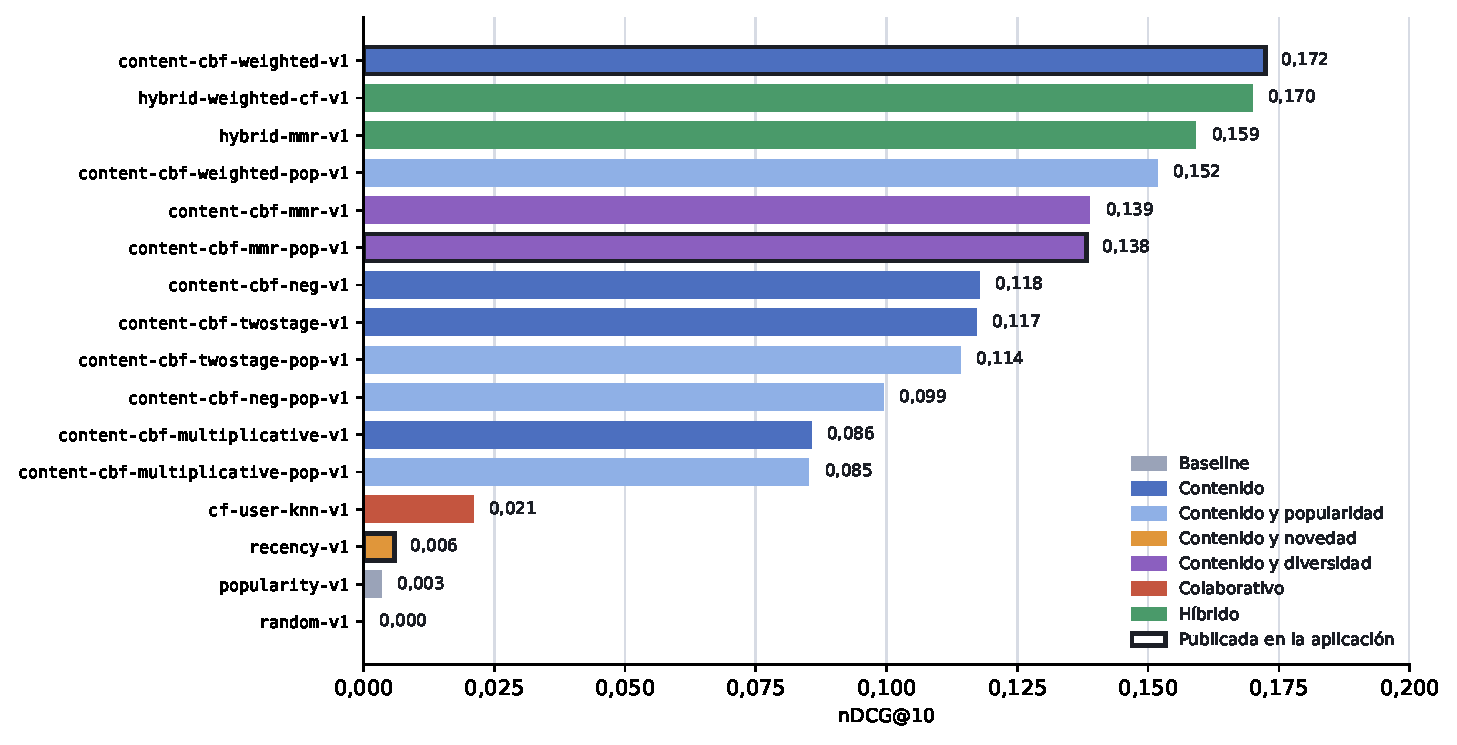
\includegraphics[width=0.9\textwidth]{figures/ndcg-algoritmos.pdf}
    \caption{\(nDCG@10\) de los dieciséis algoritmos en la evaluación v15 (\texttt{fs-v12}), por familia. El borde grueso marca las tres variantes publicadas en la aplicación.}
    \label{fig:ndcg-algoritmos}
\end{figure}

nDCG y MAP resumen la recuperación en una única cifra por algoritmo, pero no responden
directamente a la pregunta más intuitiva: ¿a cuántas personas le funcionó? La
Tabla~\ref{tab:exito-usuarios} lo hace explícito para \(K=10\), sobre los doscientos dos
ítems retenidos y los setenta y nueve usuarios evaluables.

\begin{table}[H]
\centering
\caption{Éxitos por algoritmo a \(K=10\): ítems retenidos recuperados sobre 202; usuarios
que recuperaron al menos uno de los suyos sobre 79.}\label{tab:exito-usuarios}
\small
\begin{tabularx}{\textwidth}{@{}>{\ttfamily\raggedright\arraybackslash}X C{0.22\textwidth} C{0.25\textwidth}@{}}
\textnormal{Algoritmo} & \textnormal{Ítems@10 (/202)} & \textnormal{Usuarios\(\geq\)1@10 (/79)} \\
\hline
content-cbf-weighted-v1 & 48 & 39 (49\,\%) \\
hybrid-weighted-cf-v1 & 48 & 38 (48\,\%) \\
hybrid-mmr-v1 & 42 & 35 (44\,\%) \\
content-cbf-weighted-pop-v1 & 38 & 34 (43\,\%) \\
content-cbf-mmr-v1 & 36 & 32 (41\,\%) \\
content-cbf-neg-v1 & 34 & 28 (35\,\%) \\
cf-user-knn-v1 & 7 & 7 (9\,\%) \\
popularity-v1 & 2 & 2 (3\,\%) \\
recency-v1 & 1 & 1 (1\,\%) \\
random-v1 & 0 & 0 (0\,\%) \\
\end{tabularx}
\end{table}

Leída así, la mejor variante de contenido devuelve al menos uno de los juegos retenidos del
usuario, dentro de las diez primeras posiciones, casi a la mitad de las personas evaluables
(49\,\%), frente al 9\,\% del colaborativo puro y el 3\,\% o menos de los métodos de referencia; a
\(K=20\) esa cifra sube al 58\,\% para \texttt{content-cbf-weighted-v1} (cuarenta y seis de
setenta y nueve usuarios). Esta tasa de éxito por usuario y el \(nDCG@10\) de la
Tabla~\ref{tab:resultados-ndcg10} miden cosas distintas y no deben confundirse: la primera
cuenta aciertos binarios por persona, mientras que la segunda además descuenta la posición
exacta del acierto dentro de la lista, por lo que una tasa de éxito alta no implica un nDCG
igual de alto si los aciertos tienden a aparecer hacia el final del top-\(K\) en vez de al
principio.

\section{Significación estadística}\label{sec:exp-significacion}

Las diferencias de la Tabla~\ref{tab:resultados-ndcg10} se sometieron a contraste antes de
interpretarlas, con una cadena de pruebas pensada para el caso en que dieciséis algoritmos se
miden sobre exactamente los mismos setenta y nueve usuarios (medidas repetidas, no muestras
independientes) y se quiere comparar cada par sin inflar el número de falsos positivos que
salen solo por probar muchas comparaciones a la vez. La cadena tiene cuatro piezas, todas ellas
procedimientos estadísticos estándar aplicados a este problema concreto, no invenciones del
proyecto.

Primero, una prueba de \textbf{Friedman} sirve de ómnibus: comprueba, con un único contraste,
si existe alguna diferencia entre los dieciséis algoritmos antes de gastar el presupuesto de
comparaciones en mirar pares sueltos. Es no paramétrica (no asume que los valores de nDCG se
distribuyan de forma normal, algo que no se puede dar por hecho con solo setenta y nueve
observaciones) y adecuada para medidas repetidas: cada usuario aporta una clasificación entre los
dieciséis algoritmos; la prueba contrasta si esas clasificaciones son consistentes entre sí. Sobre
\(nDCG@10\), rechaza la hipótesis de igualdad con \(\chi^2=258{,}07\) y
\(p=2{,}69\times10^{-46}\).

Segundo, confirmada la existencia de alguna diferencia, cada uno de los ciento veinte pares
posibles de algoritmos se contrasta con una prueba de \textbf{Wilcoxon de rangos con signo
pareada}: para cada usuario se calcula la diferencia de \(nDCG@10\) entre los dos algoritmos
del par; la prueba comprueba si esas diferencias pareadas se alejan de cero de forma
consistente, sin asumir tampoco su distribución. Es la elección natural aquí porque los dos
algoritmos de cada par se miden sobre las mismas setenta y nueve personas, no sobre grupos
distintos.

Tercero, probar ciento veinte pares a la vez con un umbral \(p<0{,}05\) fijo produciría, solo
por azar, varios falsos positivos aunque ningún algoritmo fuera realmente distinto de otro
(el problema de comparaciones múltiples). La \textbf{corrección de Holm} ajusta el umbral de
significación de cada una de las ciento veinte comparaciones, ordenadas de menor a mayor \(p\)
sin corregir, de forma escalonada y más potente que una corrección de Bonferroni simple sin
dejar de controlar el error de tipo I acumulado. Cincuenta y cuatro de las ciento veinte
comparaciones siguen siendo significativas después de este ajuste.

Cuarto, además del contraste de hipótesis, el artefacto conserva un \textbf{intervalo de
confianza por remuestreo BCa} (corregido por sesgo y acelerado, dos mil
remuestreos, confianza del 95\,\%, semilla fija) para el \(nDCG@10\) de cada algoritmo, que da
un rango de valores plausibles en lugar de una única cifra puntual y no exige asumir ninguna
forma concreta para la distribución del estadístico. La Tabla~\ref{tab:significacion} recoge
las comparaciones por pares más relevantes para la narrativa de este capítulo; la lista
completa de las ciento veinte vive en el artefacto versionado.

\begin{table}[H]
\centering
\caption{Comparaciones por pares más relevantes sobre \(nDCG@10\), con corrección de Holm
sobre las ciento veinte comparaciones totales.}\label{tab:significacion}
\small
\begin{tabularx}{\textwidth}{@{}Yrr@{}}
\textnormal{Comparación} & \textnormal{\(\Delta\) nDCG@10} & \textnormal{\(p\) ajustado} \\
\hline
content-cbf-weighted-v1 frente a random-v1 & +0{,}1725 & 0{,}00001 \\
content-cbf-weighted-v1 frente a popularity-v1 & +0{,}1691 & 0{,}00001 \\
hybrid-weighted-cf-v1 frente a random-v1 & +0{,}1699 & 0{,}00001 \\
cf-user-knn-v1 frente a content-cbf-weighted-v1 & \(-\)0{,}1515 & 0{,}00004 \\
cf-user-knn-v1 frente a hybrid-weighted-cf-v1 & \(-\)0{,}1489 & 0{,}00004 \\
\end{tabularx}
\end{table}

Dos lecturas se derivan de este contraste. La primera es que tanto las variantes de contenido
como los híbridos superan a los dos métodos de referencia y a \texttt{recency-v1} con significación
sobrada, lo que sí permite descartar el azar como explicación de esas diferencias concretas,
bajo este corpus y esta población. La segunda, nueva en este protocolo frente a versiones
anteriores, es que el colaborativo puro (\texttt{cf-user-knn-v1}) resulta significativamente
peor que ocho de las diez variantes de contenido, una diferenciación que la potencia
estadística de protocolos previos no alcanzaba a establecer con esta claridad. Esa lectura
tiene un matiz importante: esta prueba mide específicamente la recuperación de obras de la
etiqueta de contenido dominante del perfil de cada usuario y \texttt{cf-user-knn-v1} no usa
etiquetas en absoluto, sino similitud de patrones de valoración entre usuarios. La diferencia
es real y significativa, pero mide precisamente el terreno que la señal colaborativa no
modela; no es evidencia de que el filtrado colaborativo sea inferior en una tarea distinta,
como recuperar valoraciones de usuarios con gustos parecidos sin restricción de género. Los
híbridos combinan ambas señales en parte por esta razón: para no depender de ninguna de las
dos en solitario.

\section{Diversidad, cobertura y amenazas a la validez}\label{sec:exp-amenazas}

MMR introduce un objetivo distinto de la recuperación puntual: reducir redundancia entre elementos ya seleccionados. Sus resultados deben leerse junto con diversidad intra-lista, novedad, cobertura del catálogo, cobertura de predicción y HHI cuando el artefacto los publica. Una mejora de diversidad no compensa automáticamente una pérdida de nDCG, ni la métrica de acierto debe ocultar concentración. SavePoint mantiene estas medidas separadas para que el compromiso sea auditable. Con \(K=10\), la diversidad intra-lista de \texttt{content-cbf-weighted-v1} es 0,531 y sube a 0,652 en \texttt{content-cbf-mmr-v1}, mientras que su \(nDCG@10\) baja de 0,1725 a 0,1389; en el híbrido, de 0,532 a 0,655 de diversidad y de 0,1699 a 0,1591 de \(nDCG@10\). La cobertura es baja en todos los algoritmos: la mejor variante de contenido recomienda 241 de las 13.618 obras candidatas (el 1,77\,\%) entre los 79 usuarios y la popularidad solo 11 (el 0,08\,\%), con un HHI de 0,0988 frente a 0,0132 de la variante de contenido y de 0,0765 del colaborativo, que también concentra. La cobertura de predicción es completa (1,00) en los dieciséis algoritmos.

Las amenazas principales son población sintética, un solo consumo de la prueba y dependencia de
metadatos externos gobernados. El corpus y la versión inmutable son fortalezas de reproducibilidad,
pero acotan la generalización: la significación estadística de la Sección~\ref{sec:exp-significacion}
respalda que las diferencias observadas no son ruido bajo este corpus y esta población, no
que se sostengan sobre usuarios reales. Un estudio posterior debería incluir más semillas,
sensibilidades de hiperparámetros, datos observados con consentimiento y evaluación con
participantes, sin mutar el artefacto v15 ya publicado.

Este capítulo ha presentado la evaluación experimental de los algoritmos. El capítulo siguiente
cierra la memoria con el grado de cumplimiento de los objetivos y las líneas de continuación.
